\section{Inverse Kinematics}

With the forward kinematic equations, the position of the end effector can be determined relative to the base frame for given values of the joint variables.
In the context of robotics, it is also necessary to determine these joint variables for a given end effector position.
This is referred to as the inverse kinematic problem.
Solving the inverse kinematic problem for a given serial link actuator allows to transform a motion plan of the \ac{EOAT} into joint actuator trajectories for the robot.\\
\\
\subsection{Existence of Solutions} \label{sec:ExistSol}
To determine the joint values for a \ac{EOAT}-position it needs to be determined, if there exists a solution.
Not all positions are equally reachable.
There are two types of workspace (\cite{craig1986introduction}, chapter 4):%, p.102):
\begin{itemize}[wide=\parindent] 
	\item[\textbf{dextrous workspace}] volume of space that the robot end-effector can reach with all orientations
	\item[\textbf{reachable workspace}] volume of space, that the robot can reach in at least one orientation
\end{itemize}


A manipulator with less than 6 \ac{DOF} cannot reach all positions and orientations in 3D-space. Further limitations can be imposed by the axis alignment. A planar manipulator for example cannot reach  out of the plane. \cite{craig1986introduction}

\subsection{Multiple Solutions} \label{MultipSol}
A 6 \ac{DOF} robot has multiple sets of inverse solutions. To understand why there are multiple solutions, it helps to have a look at  \Autoref{fig:multipSol3Link}. The same end effector position and orientation can be reached in two ways by a 3-link manipulator. 

\begin{figure}[H]
	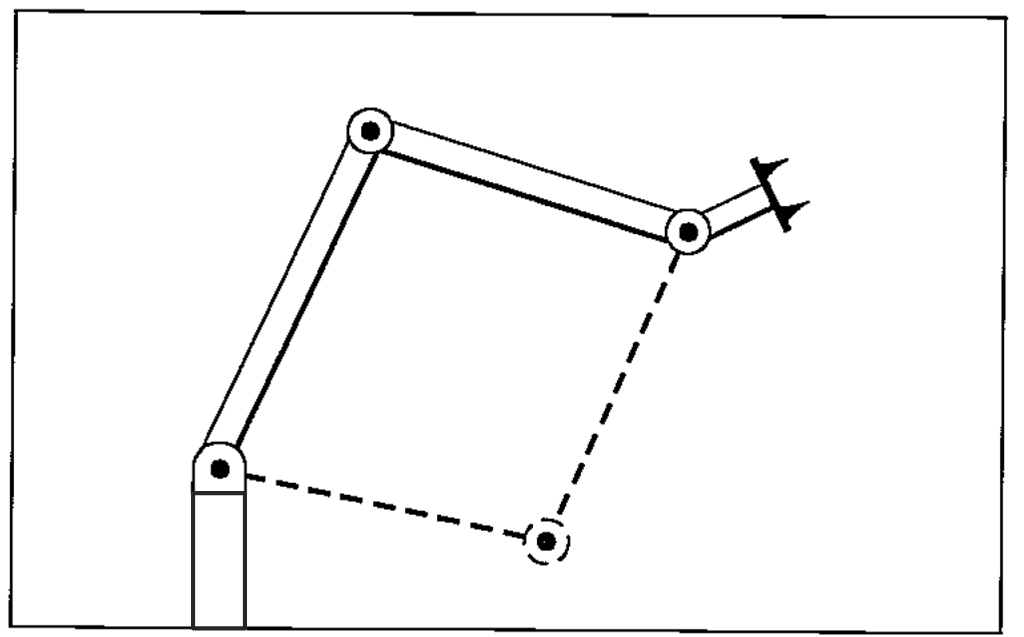
\includegraphics[
	width=0.8\linewidth,
	center,
	keepaspectratio,
	]{invKin/Multip_Sol}
	\caption{Three link manipulator with 2 solutions (see \cite{craig1986introduction}, p.103 )}
	\label{fig:multipSol3Link}
\end{figure}

This can be extended to the 6 \ac{DOF} serial link manipulators.
%As stated by YanWu et al. 
There are 8 groups of inverse solution for most \ac{EOAT}-positions within the manipulator's workspace \cite{invKinSolYanWu} for 6 \ac{DOF} manipulators with spherical wrists as seen in \Autoref{sec:SphericalVsNonspherical}. 

\begin{figure}[H]
	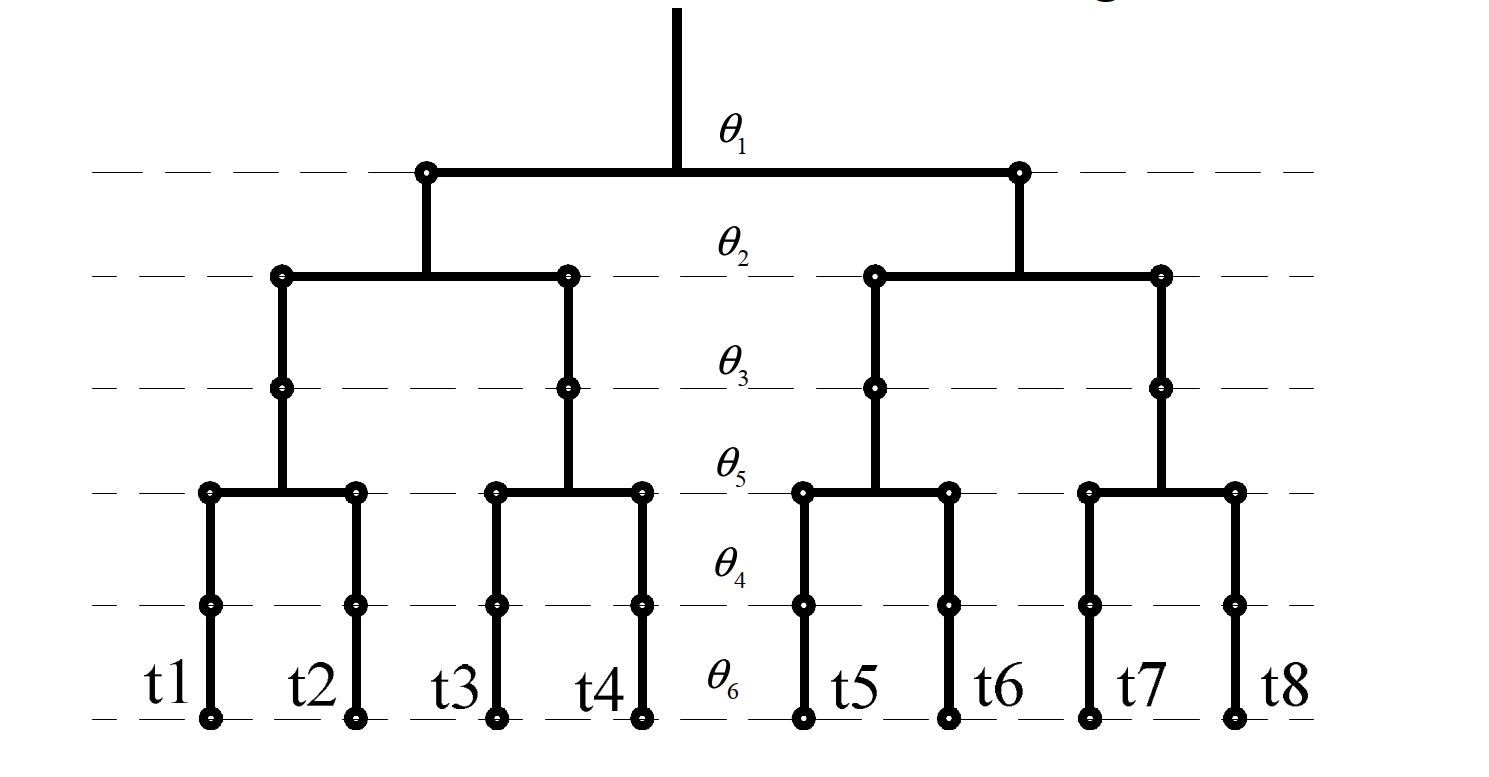
\includegraphics[
	width=1\linewidth,
	center,
	keepaspectratio,
	]{invKin/TreeOfInvserseSolution}
	\caption{Tree of inverse solutions (\cite{invKinSolYanWu}, fig.2)}
	\label{fig:invKinTree}
\end{figure}
%
The tree of inverse solutions shown in \Autoref{fig:invKinTree} is a schematic representation of different possible solutions. It does not show actual positions. A set of the different joint configurations for inverse solutions in the Fanuc can be found in \Autoref{sec:RobConf}.


\subsection{Inverse Solution of 6 \ac{DOF} Robot} \label{sec:InvSol6DOF}

As shown in \Autoref{ForKinEq} the end effector position is defined by four $3 \times 1$ vectors $[\gls{n_xyz},\gls{o_xyz},\gls{a_xyz},\gls{p_xyz}]$. With these known, the joint variables $(\theta_1, \theta_2, \theta_3, \theta_4, \theta_5, \theta_6)$ can be calculated.
This problem  is solved by the method of using the inverse transformation of unknown link pre-multiplication as presented %by Yan Wu et al.
in \cite{invKinSolYanWu}. This solution works only for 6 \ac{DOF} serial link mechanisms with spherical wrist. 
For a distinction between spherical and non-spherical wrists see \Autoref{sec:SphericalVsNonspherical}.

\paragraph{Forward kinematic equation}
For a  6 \ac{DOF} Robot, the  forward kinematic matrix equation from \ref{eq:SummofTranfMatr} and \ref{eq:matrixForm} can be reformulated into  \ref{eq:ForwKinEquMatr}.

\begin{equation}\label{eq:ForwKinEquMatr}
	^0\hat{T}_6 = \\
	\begin{bmatrix}
n_x & o_x & a_x & p_x \\
n_y & o_y & a_y & p_y \\
n_z & o_z & a_z & p_z \\
0 & 0 & 0 & 1 \\
\end{bmatrix}
=
\phantom{}^0\hat{T}_1(\theta_1)\phantom{}^1\hat{T}_2(\theta_2)\phantom{}^2\hat{T}_3(\theta_3)\phantom{}^3\hat{T}_4(\theta_4)\phantom{}^4\hat{T}_5(\theta_5)\phantom{}^5\hat{T}_6(\theta_6)\\
\end{equation}

\subsection{The Inverse Solution} \label{InverseSol}
With $[\gls{n_xyz},\gls{o_xyz},\gls{a_xyz},\gls{p_xyz}]$ known, the angle values of the joint variables can be determined by separation of the joint variables. 
As stated in \Autoref{MultipSol}, there are two solutions for each $\theta_i$. Steps on how to obtain these equations can be found in \Autoref{sec:InvKinEqSteps}.
\medskip


\begin{subequations}\label{eq:BackKinEquations_shortIntext}
	\begin{align}
			\theta_{1_1} &= \atantwo ( p_y - a_y d_6 , p_x - a_x d_6) 
		\phantom{..........}
		\theta_{1_2} = \atantwo (-p_y + a_y d_6 ,-p_x + a_x d_6) \label{eq:BackKinEquations_shortIntext_1} \\
		\theta_{2_{1/2}} &= \atantwo (-v , u)\pm \atantwo(\sqrt{v^2 +u^2 - m^2 } m) \\
		\theta_{3_{1/2}} &= \atantwo(-d_4 , a_3) \pm \atantwo (2 (\sqrt{d_4^2 +a_3^2 -h^2} h)) \\
		\theta_{5_{1/2}} &= \pm \acos [ ( -c_1 s_2 a_x - s_1 s_2 a_y - c_2 a_z) c_3 - (c_1 c_2 a_x + s_1 c_2 a_y - s_2 a_z) s_3] \\
		\theta_{4_{1/2}} &= \pm \arccos [ \frac{ c_1 c_2 a_x + s_1 c_2 a_y - s_2 a_z + s_3 c_5}{-c_3 s_5}] \\
		\theta_{6_{1/2}} &= \atantwo(s_1 n_x -c_1 n_y , s_1 o_x -c_1 o_y) \pm \atantwo(\sqrt{(s_1 n_x - c_1 n_y)^2 + (s_1 o_x - c_1 o_y )^2 - c_4^2}  c_4) 
	\end{align}
\end{subequations}





%\paragraph{$\pmb{\theta_1}$:}
%
%
%\begin{multline}\label{eq:sol_theta_1}
%	\theta_{1_1} = \atantwo ( p_y - a_y d_6 , p_x - a_x d_6) 
%	\phantom{..........}
%	\theta_{1_2} = \atantwo (-p_y + a_y d_6 ,-p_x + a_x d_6) 
%\end{multline}
%\medskip
%
%\paragraph{$\pmb{\theta_2}$:}
%
%
%\begin{equation}\label{eq:sol_theta_2}
%	\theta_{2_{1/2}} = \atantwo (-v , u)\pm \atantwo(\sqrt{v^2 +u^2 - m^2 } m)
%\end{equation}
%
%
%
%\paragraph{$\pmb{\theta_3}$:}
%
%
%\begin{equation}\label{eq:sol_theta_3}
%	\theta_{3_{1/2}} = \atantwo(-d_4 , a_3) \pm A \tan (2 (\sqrt{d_4^2 +a_3^2 -h^2} h))
%\end{equation}
%
%
%\paragraph{$\pmb{\theta_5}$:}
%
%
%
%\begin{equation}\label{eq:sol_theta_5}
%	\theta_{5_{1/2}} = \pm \acos [ ( -c_1 s_2 a_x - s_1 s_2 a_y - c_2 a_z) c_3 - (c_1 c_2 a_x + s_1 c_2 a_y - s_2 a_z) s_3]
%\end{equation}
%
%\paragraph{$\pmb{\theta_4}$:}
%
%
%\begin{equation}\label{eq:sol_theta_4}
%	\theta_{4_{1/2}} = \pm \arccos [ \frac{ c_1 c_2 a_x + s_1 c_2 a_y - s_2 a_z + s_3 c_5}{-c_3 s_5}]
%\end{equation}
%
%\paragraph{$\pmb{\theta_6}$:}
%
%
%\begin{equation}\label{eq:sol_theta_6}
%	\theta_{6_{1/2}} = \atantwo(s_1 n_x -c_1 n_y , s_1 o_x -c_1 o_y) \pm \atantwo(\sqrt{(s_1 n_x - c_1 n_y)^2 + (s_1 o_x - c_1 o_y )^2 - c_4^2}  c_4)
%\end{equation}

\medskip

Following middle variables have been chosen:

\begin{subequations}
	\begin{align*}
		u&=c_1 (p_x d_6 a_x ) + s_1 (p_y -a_y d_6)-a_1 \\
		v&= p_z - a_z d_6 \\
		m&= \frac{a_3^2 +d_4^2 - u^1 -v^2 - a_2^2}{-2a_2} \\
		h&=-\frac{a_3^2 + d_4^2 - u^2 -v^2 + a_2^2}{2a_2} .
	\end{align*}
\end{subequations}

Following notation is used: $c_i = cos(\theta_i)$.


%\begin{equation}
%u=c_1 (p_x d_6 a_x ) + s_1 (p_y -a_y d_6)-a_1 
%\end{equation}
%\begin{equation}
%v= p_z - a_z d_6
%\end{equation}
%\begin{equation*}
%m = \frac{a_3^2 +d_4^2 - u^1 -v^2 - a_2^2}{-2a_2}
%\end{equation*}
%\begin{equation*}
%h=-\frac{a_3^2 + d_4^2 - u^2 -v^2 + a_2^2}{2a_2}
%\end{equation*}


With \Autoref{eq:BackKinEquations_shortIntext} %\ref{eq:sol_theta_1},\ref{eq:sol_theta_2},\ref{eq:sol_theta_3},\ref{eq:sol_theta_4},\ref{eq:sol_theta_5} and \ref{eq:sol_theta_6} \ref{eq:sol_theta_1} to \ref{eq:sol_theta_6} 
the values for $\theta_1$ to %, \theta_2, \theta_3, \theta_4, \theta_5, 
$\theta_6$ can be calculated for all reachable end effector positions.\\

\medskip


\subsection{Optimization of Inverse Kinematic Solution}

As seen in \Autoref{sec:ExistSol} there exist eight sets of inverse solutions in the dextrous workspace.
The optimal set of solutions can be found through an optimization function. 
This optimization function needs to find the set of solution that can reach the desired position fastest from the current position.\\
\\
\paragraph{Cost function}
Equation \Autoref{eq:costFuncinvOptim} is the cost function to be minimized. It calculates the total sum of angular distance $(err)$ for a given target angle $\theta_i (k+1)$ and departing angle $\theta_i(k)$.
%\begin{itemize}[wide=\parindent] 
%	\item[$\theta_i (k+1)$:] target angle
%	\item[$\theta_i(k)$:] departing angle
%	\item[$k_i$:] power value
%\end{itemize}

\begin{equation}\label{eq:costFuncinvOptim}
	err =  \min\sum_{i=1}^{6} k_i [\theta_i (k+1) - \theta_i(k)] 
\end{equation}

As can be seen, this cost function minimizes the sum of angles over all axes for the movement of the end effector from position $[n_i,o_i,a_i,p_i ]$ to $[n_{i+1}, o_{i+1}, a_{i+1}, p_{i+1}]$ by using the inverse solution presented in \Autoref{InverseSol}.

%\paragraph{Limitations of cost function}
%This cost function not necessarily gives the fastest path, as it does not account for the actual movement speed of the different axes. 
%A possible solution for this would require multiplying with a cost factor between 0 and 1 for each joint ( 1 for the slowest joint) with the respective angle error to account for the difference in angular velocity.

\paragraph{Accounting for motor torque}
With the power value $k_i$, the cost function accounts for different maximum speeds, power ratings and gear boxes on each axis. It is a cost factor between 0 and 1 for each joint ( 1 for the slowest joint) that is multiplied with the respective angle error to account for the difference in angular velocity. 



\paragraph{Description of implementation}

An implementation of this function receives the current position either in joint angles or Cartesian coordinates of the end-effector %which could be given in form of a rotation matrix as seen in \ref{eq:matrixForm} or in form of euclidean space $[x,y,z, \alpha, \beta, \gamma]$ which could be transformed by the inverse of \ref{eq:rotMatrix_composition} into a rotation matrix.

This algorithm would then start the calculation to get all possible paths in the tree of inverse solutions (see \Autoref{fig:invKinTree}) for position ${i+1}$.

\paragraph{Algorithm for minimal computational effort}

To minimize the computational effort, following algorithm is proposed %by Yan Wu et al. 
in \cite{invKinSolYanWu}:

\begin{enumerate}
	\item The calculation starts with $\theta_1$ by finding the two solutions for equation \Autoref{eq:BackKinEquations_shortIntext_1}.
	\item When calculating $\theta_2$:
	\begin{enumerate}
		\item  The term $ v^2 + u^2 - m^2 $ should be $ > 0$, otherwise the program can terminate the calculation of the subsequent steps of this group, return $err = inf $ or $NaN $ , and provide a variable like $P=1$ to determine the cause for the abortion of subsequent steps
		\item If there is a solution for $\theta_2$ it needs to be tested for \glspl{ExtraneousRoot}
		%An extraneous root is  introduced into an equation in the process of solving another equation, but is not a solution of the equation to be solved \cite{extraneousroot}. This test is done simply by substituting the solution for $\theta_2$ into the original equation \ref{eq:1-4+2_4}. If an extraneous root is found, the program can terminate and return $err = inf$ or $ NaN$  and $P=2$ for cause of abortion. 
	\end{enumerate}
	\item If the calculation has been continued, $\theta_3$ can be determined. Again a test for \glspl{ExtraneousRoot} is necessary
	\item When calculating $\theta_5$, test for \glspl{ExtraneousRoot}
	\item When calculating $\theta_4$, test for \glspl{ExtraneousRoot}
	\item calculate $\theta_6$
	\item determine error as seen in \Autoref{eq:costFuncinvOptim} for all possible paths
	\item find $\min ( err(t_1^8))$ 
\end{enumerate}

The resulting set of angle values is the output of the algorithm. It is the unique inverse solution, determined easiest to reach with the given cost function in \Autoref{eq:costFuncinvOptim}. 





%https://robotics.stackexchange.com/questions/10322/is-it-possible-to-get-all-possible-solutions-of-verse-kinematics-of-a-6-dof-ar
%In general, if the wrist is spherical (i.e., all three axes intersect), you can enumerate all of the various closed-form solutions through a method known as wrist partitioning. This method uses the three arm joints to solve for the position of the wrist center. It then uses the wrist joints to determine the joint angles which orient the end effector properly. Multiple solutions are possible from "wrist up" and "wrist down" options, "elbow up" and "elbow down" options (for an articulated arm), and "over the shoulder" options also. For other robot geometries the options would differ.

%If the wrist is not spherical, it becomes quite challenging to find a closed-form inverse solution. But you still have the various geometric options for inverse kinematics solutions.
%
%One way to make sure you are identifying all of the solutions is to recall the fundamentals of trigonometry. Recall that sin(θ)=−sin(−θ)
%and cos(θ)=cos(−θ). So when you are solving for θ you have to consider the other angles which produce the same result using these and other trigonometric identities. 